\chapter{Similariteitsmaten voor beelden}

Een similariteitsmaat voor beelden is een maat die de gelijkenis tussen twee gegeven
beelden uitdrukt als een getal uit het interval $[0,1]$. Dit getal nadert naar 1
naarmate de gelijkenis groter is. Bijgevolg kunnen we een dergelijke maat gebruiken om
een lijst van zoekresultaten te herordenen volgens similariteit met een bepaald 
voorbeeld-beeld uit die lijst. 

We construeren een similariteitsmaat voor beelden in twee stappen. Eerst identificeren we
een beeld, al dan niet rechtstreeks, met een (L-)vaagverzameling. Daarna maken we gebruik van
de vaagsimilariteitsmaten uit \ref{sectie:vaagsimilariteitsmaten} om deze (L-)vaagverzamelingen te
vergelijken. 

In het vervolg van deze scriptie bedoelen we met de term ``similariteitsmaat'' steeds
een similariteitsmaat voor beelden. Dit omvat dus zowel een manier van identificeren als een 
vaagsimilariteitsmaat.

\section{Eigenschappen}

In de volgende hoofdstukken construeren we een aantal similariteitsmaten voor beelden. Hierbij 
eisen we dat al onze similariteitsmaten \emph{reflexief} en \emph{symmetrisch} zijn.

\subsection{Reflexiviteit}

Voor twee identieke beelden verwachten we dat een similariteitsmaat $M$ als output $1$
teruggeeft. Met andere woorden, voor een beeld $A$ moet gelden: $M(A,A)=1$.
Deze eigenschap heeft als gevolg dat het voorbeeld-beeld zich steeds vooraan in
de geordende lijst van zoekresultaten moet bevinden.

\subsection{Symmetrisch}

De output van een similariteitsmaat $M$ wordt verwacht onafhankelijk te zijn van de 
volgorde waarin de beelden aangeboden worden. Voor beelden $A$ en $B$ moet dus gelden:
$M(A,B)=M(B,A)$.

\section{Evaluatie van performantie}

\subsection{Globale genormaliseerde gemiddelde rang (GGGR)}

Om uit meerdere similariteitsmaten de meest geschikte te kiezen, 
moeten we een manier vinden om een dergelijke maat objectief te beoordelen. 
Dit zullen we doen door elke
maat, voor een bepaald voorbeeld-beeld, toe te passen op een eenzelfde collectie 
van beelden. Vervolgens zullen we de rangschikking die we zo bekomen
beoordelen met behulp van een performantiemaat.

Figuur~\ref{fig:testcollectie} bevat de collectie van beelden die we gaan 
gebruiken. Deze collectie bestaat uit een selectie van beelden uit
de \emph{Columbia object image library} \cite{coil-100}. Deze bibliotheek van beelden 
werd gegenereerd 
door een aantal roterende objecten op bepaalde vaste momenten te fotograferen. 
Onze testcollectie bestaat uit foto's van elf objecten. Van elke object zijn
er zes momentopnames, wat een totaal van $11 \cdot 6 = 66$ beelden geeft.

\begin{figure}[p]
\begin{center}

\begin{tabular}{cccccc}

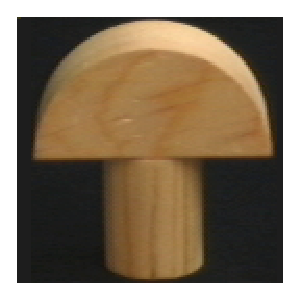
\includegraphics[width=2cm]{coil/beeld-0.eps} &
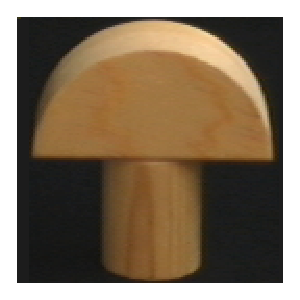
\includegraphics[width=2cm]{coil/beeld-1.eps} &
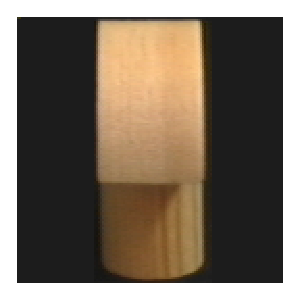
\includegraphics[width=2cm]{coil/beeld-2.eps} &
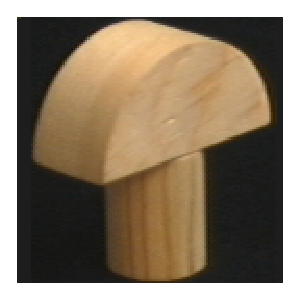
\includegraphics[width=2cm]{coil/beeld-3.eps} &
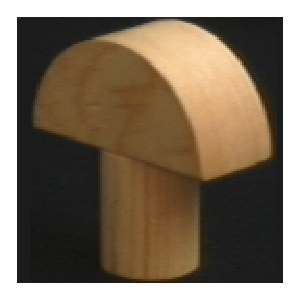
\includegraphics[width=2cm]{coil/beeld-4.eps} &
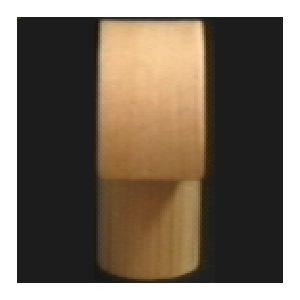
\includegraphics[width=2cm]{coil/beeld-5.eps} \\

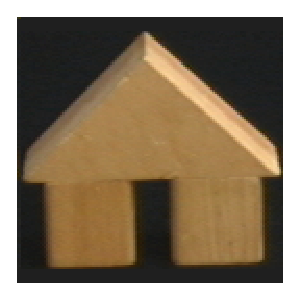
\includegraphics[width=2cm]{coil/beeld-42.eps} &
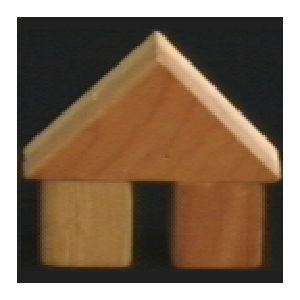
\includegraphics[width=2cm]{coil/beeld-43.eps} &
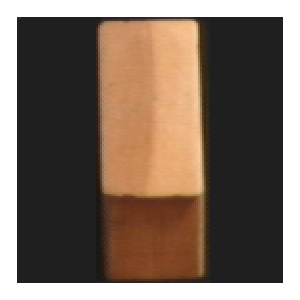
\includegraphics[width=2cm]{coil/beeld-44.eps} &
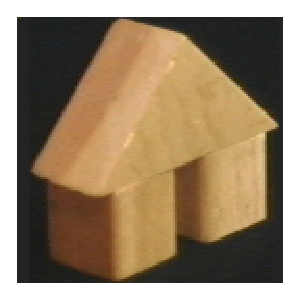
\includegraphics[width=2cm]{coil/beeld-45.eps} &
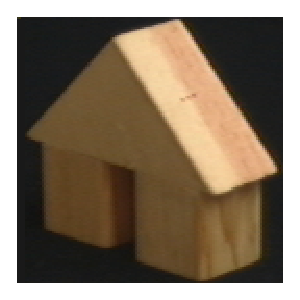
\includegraphics[width=2cm]{coil/beeld-46.eps} &
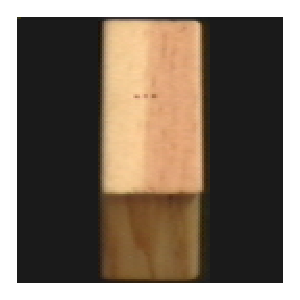
\includegraphics[width=2cm]{coil/beeld-47.eps} \\

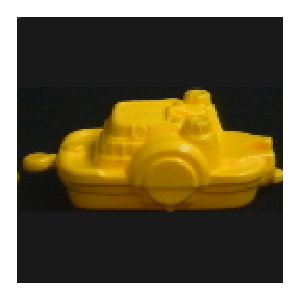
\includegraphics[width=2cm]{coil/beeld-12.eps} &
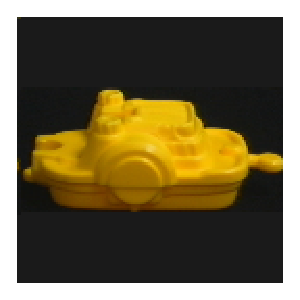
\includegraphics[width=2cm]{coil/beeld-13.eps} &
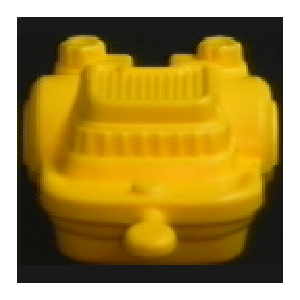
\includegraphics[width=2cm]{coil/beeld-14.eps} &
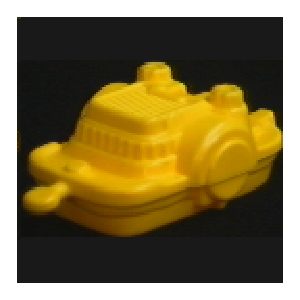
\includegraphics[width=2cm]{coil/beeld-15.eps} &
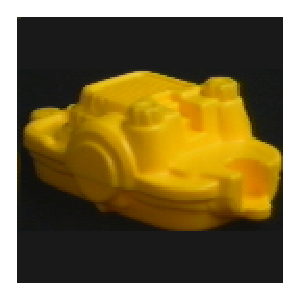
\includegraphics[width=2cm]{coil/beeld-16.eps} &
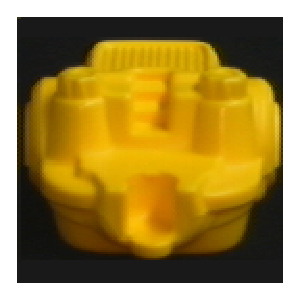
\includegraphics[width=2cm]{coil/beeld-17.eps} \\

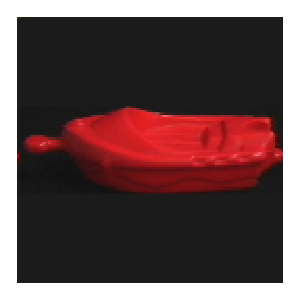
\includegraphics[width=2cm]{coil/beeld-18.eps} &
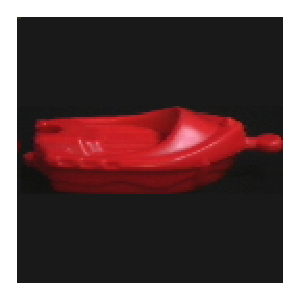
\includegraphics[width=2cm]{coil/beeld-19.eps} &
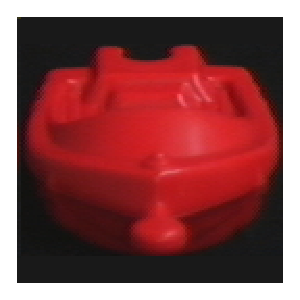
\includegraphics[width=2cm]{coil/beeld-20.eps} &
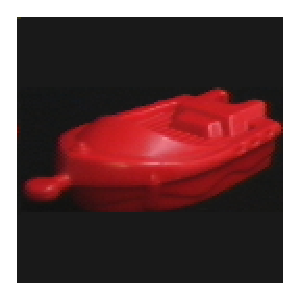
\includegraphics[width=2cm]{coil/beeld-21.eps} &
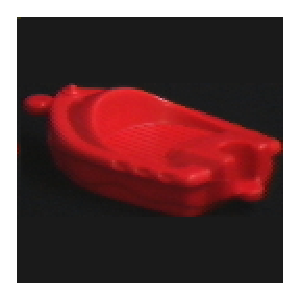
\includegraphics[width=2cm]{coil/beeld-22.eps} &
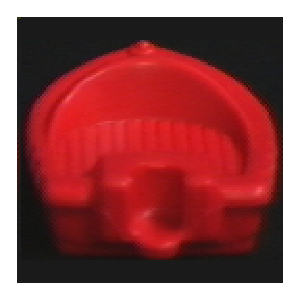
\includegraphics[width=2cm]{coil/beeld-23.eps} \\

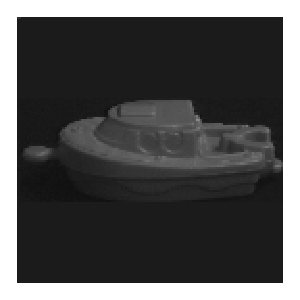
\includegraphics[width=2cm]{coil/beeld-24.eps} &
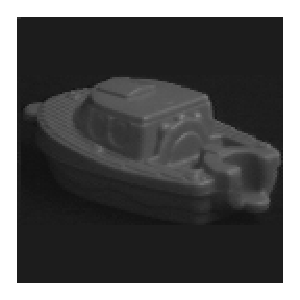
\includegraphics[width=2cm]{coil/beeld-25.eps} &
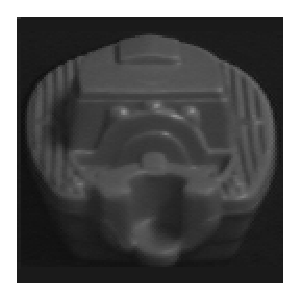
\includegraphics[width=2cm]{coil/beeld-26.eps} &
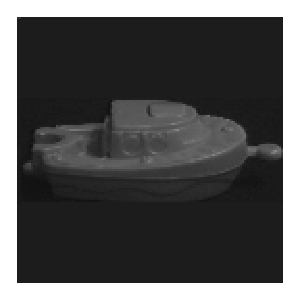
\includegraphics[width=2cm]{coil/beeld-27.eps} &
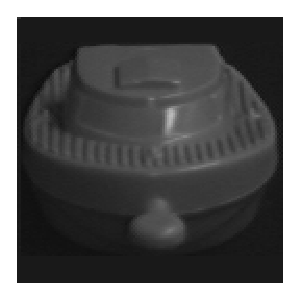
\includegraphics[width=2cm]{coil/beeld-28.eps} &
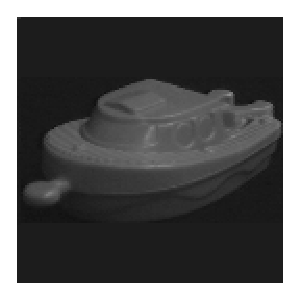
\includegraphics[width=2cm]{coil/beeld-29.eps} \\

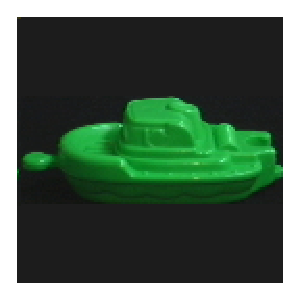
\includegraphics[width=2cm]{coil/beeld-54.eps} &
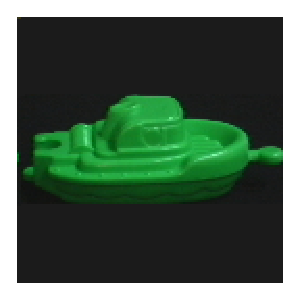
\includegraphics[width=2cm]{coil/beeld-55.eps} &
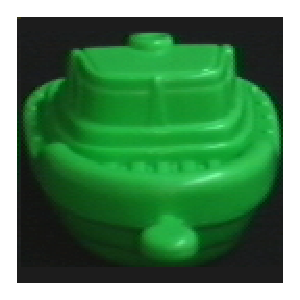
\includegraphics[width=2cm]{coil/beeld-56.eps} &
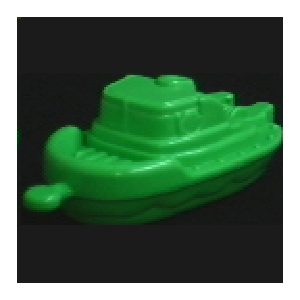
\includegraphics[width=2cm]{coil/beeld-57.eps} &
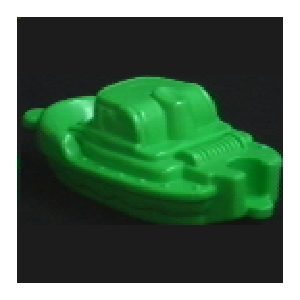
\includegraphics[width=2cm]{coil/beeld-58.eps} &
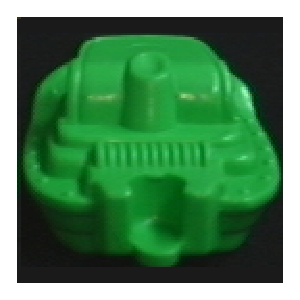
\includegraphics[width=2cm]{coil/beeld-59.eps} \\

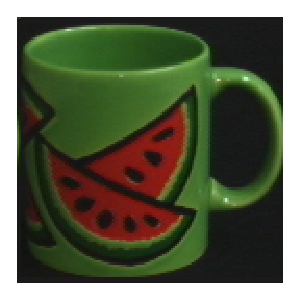
\includegraphics[width=2cm]{coil/beeld-30.eps} &
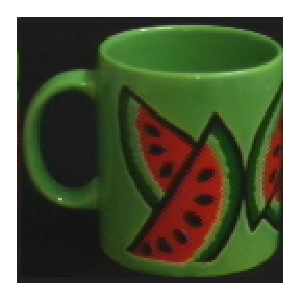
\includegraphics[width=2cm]{coil/beeld-31.eps} &
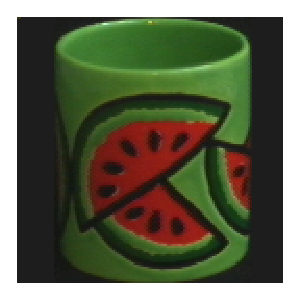
\includegraphics[width=2cm]{coil/beeld-32.eps} &
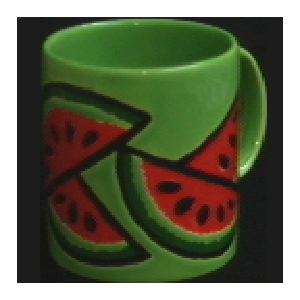
\includegraphics[width=2cm]{coil/beeld-33.eps} &
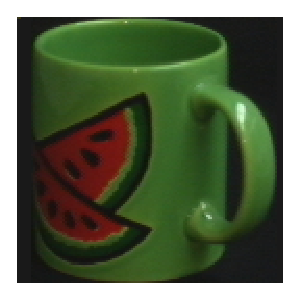
\includegraphics[width=2cm]{coil/beeld-34.eps} &
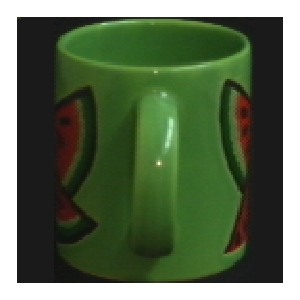
\includegraphics[width=2cm]{coil/beeld-35.eps} \\

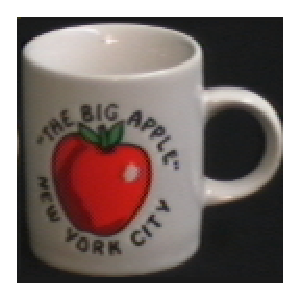
\includegraphics[width=2cm]{coil/beeld-36.eps} &
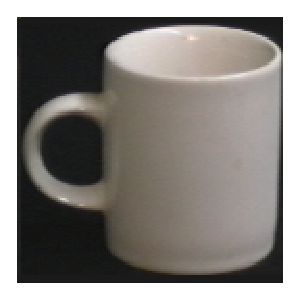
\includegraphics[width=2cm]{coil/beeld-37.eps} &
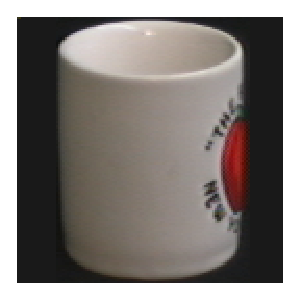
\includegraphics[width=2cm]{coil/beeld-38.eps} &
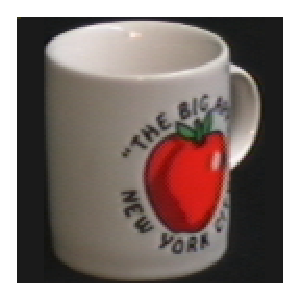
\includegraphics[width=2cm]{coil/beeld-39.eps} &
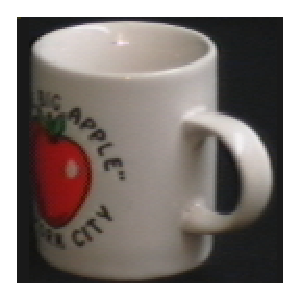
\includegraphics[width=2cm]{coil/beeld-40.eps} &
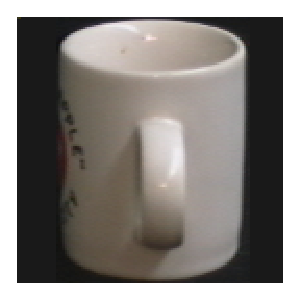
\includegraphics[width=2cm]{coil/beeld-41.eps} \\

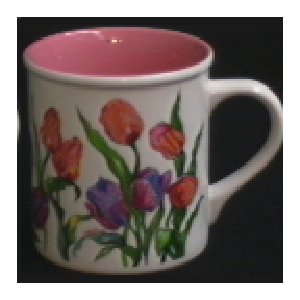
\includegraphics[width=2cm]{coil/beeld-6.eps} &
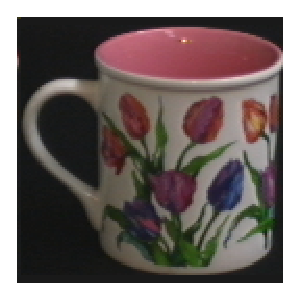
\includegraphics[width=2cm]{coil/beeld-7.eps} &
\includegraphics[width=2cm]{coil/beeld-8.eps} &
\includegraphics[width=2cm]{coil/beeld-9.eps} &
\includegraphics[width=2cm]{coil/beeld-10.eps} &
\includegraphics[width=2cm]{coil/beeld-11.eps} \\

\includegraphics[width=2cm]{coil/beeld-48.eps} &
\includegraphics[width=2cm]{coil/beeld-49.eps} &
\includegraphics[width=2cm]{coil/beeld-50.eps} &
\includegraphics[width=2cm]{coil/beeld-51.eps} &
\includegraphics[width=2cm]{coil/beeld-52.eps} &
\includegraphics[width=2cm]{coil/beeld-53.eps} \\

\includegraphics[width=2cm]{coil/beeld-60.eps} &
\includegraphics[width=2cm]{coil/beeld-61.eps} &
\includegraphics[width=2cm]{coil/beeld-62.eps} &
\includegraphics[width=2cm]{coil/beeld-63.eps} &
\includegraphics[width=2cm]{coil/beeld-64.eps} &
\includegraphics[width=2cm]{coil/beeld-65.eps} \\

\end{tabular}
\caption{\label{fig:testcollectie}De gebruikte collectie van beelden.}
\end{center}
\end{figure}

Voor het beoordelen van een rangschikking, gebruiken we de \emph{genormaliseerde gemiddelde rang} 
(GGR) \cite{muller:perf_eval}. Deze performantiemaat wordt toegepast op een collectie
van $N$ beelden. Voor elk van deze beelden bevat de collectie
$N_R$ zogenaamde \emph{relevante beelden}. In het geval van onze testcollectie geldt $N = 66$.
We gaan er in deze collectie vanuit dat foto's van eenzelfde object relevant zijn ten opzichte
van elkaar: $N_R = 6$. Beschouw nu de vector 
$(r_1,r_2,\ldots,r_{N_R}) \in \{1,2,\ldots,N\}^{N_R}$, waarbij $r_i$ het
rangnummer van het $i$-de relevante beeld voorstelt. De performantiemaat
wordt dan als volgt gedefinieerd:
\begin{definitie}
De genormaliseerde gemiddelde rang wordt gegeven door de volgende afbeelding:
$$
\begin{array}{lrcl}
\textrm{GGR}: 	& \{1,2,\ldots,N\}^{N_R} & \to 	& [0,1] \\
		& (r_1,r_2,\ldots,r_{N_R}) & \mapsto &
	{\displaystyle\frac{1}{N \cdot N_R}\left[ \left(\sum_{i=1}^{N_R}r_i\right) - \frac{N_R \cdot (N_R + 1)}{2} \right]},\\[15pt]
	& & & \qquad \quad \forall (r_1, r_2, ..., r_{N_R}) \in \{1,2,\ldots,N\}^{N_R}
\end{array}
$$
\end{definitie}
\noindent
Deze maat nadert naar 1 naarmate de performantie slechter wordt.

Tot nu toe hebben we er echter nog geen rekening mee gehouden dat de performantie van
een similariteitsmaat afhankelijk kan zijn van het gekozen voorbeeld. Dit probleem lossen we
op door de GGR te berekenen voor meerdere voorbeelden en het gemiddelde van de bekomen waarden
te beschouwen. We kiezen hierbij de beelden uit de linker kolom van 
figuur~\ref{fig:testcollectie} als voorbeeld. De waarde die we zo bekomen noemen we de
\emph{globale genormaliseerde gemiddelde rang} (GGGR). Het is deze waarde die we zullen gebruiken
om de performantie van een similariteitsmaat te evalueren. We zullen dus met andere woorden op
zoek gaan naar similariteitsmaten waarvan de GGGR zo klein mogelijk is.

\subsection{Rekentijd}

We zullen voor elke similariteitsmaat die we construeren ook meten hoelang het duurt om
de rangschikkingen, die nodig zijn om de GGGR te bepalen, te berekenen. Aan deze 
rekentijd hechten we echter niet zoveel belang als aan de GGGR, vermits het in onze
praktische implementatie niet absoluut noodzakelijk is dat de similariteitsmaten zo weinig
mogelijk rekentijd vereisen. De collecties van beelden waarop ze daar toegepast worden
zijn immers beperkt in grootte. Bovendien worden de berekeningen aan de kant van de client
uitgevoerd, waardoor er geen gevaar is voor overbelasting van de server.

